\sect{7.4\quad 断路复形}
设 $M=M(S,\omega)$ 是有序拟阵。回忆：从回路中删去最小元素，所得集合称为断路。$S$ 中所有不含断路的子集组成的单纯复形记为 $\BC_\omega(M)$，称为 $M$ 的\textbf{断路复形}。注意它有定义当且仅当 $M$ 无环；若有环，则每个子集都含断路 $\varnothing$。
讨论断路复形时，除环外，方便时也可排除平行元素。无环拟阵中若 $r_M(\{x,y\})=1$，称 $x,y$ 平行。平行是等价关系。在等价类集 $\bar S$ 上定义秩函数 $r_{\bar M}(\{X_1,\ldots,X_n\})=r_M(X_1\cup\cdots\cup X_n)$，得到无环且无平行元素的拟阵 $\bar M(\bar S)$，称为 $M$ 的\textbf{简化}。若 $M(S,\omega)$ 有序，按各平行类的最小元素给 $\bar S$ 排序，记为 $\bar\omega$。有如下直接观察：
\st{命题7.4.1}断路复形 $\BC_\omega(M)$ 与 $\BC_{\bar\omega}(\bar M)$ 同构。\qed
需要解释次序在构造中的作用：同一拟阵的不同点序，可能给出不同构的断路复形，例7.4.4将予以展示；但其重要不变量与次序无关。
设无环有序拟阵 $M(S,\omega)$ 的最小元素为 $e$。$S-e$ 中所有不含断路的子集组成\textbf{约化断路复形}，记为 $\overline{\BC}_\omega(M)$。先列出基本观察。
\st{命题7.4.2}设 $M(S,\omega)$ 无环且秩为 $r$。则：
\begin{enumerate}[label=(\roman*)]
\item $\overline{\BC}_\omega(M)\subseteq\BC_\omega(M)\subseteq\IN(M)$；
\item $\BC_\omega(M)$ 是纯 $(r-1)$ 维复形，其刻面为 $M$ 的nbc基；
\item $\BC_\omega(M)$ 是以 $e$ 为锥顶、以 $\overline{\BC}_\omega(M)$ 为底的锥；
\item $\overline{\BC}_\omega(M)$ 是纯 $(r-2)$ 维复形。
\end{enumerate}
\pr 若 $X\subseteq S$ 不含断路，则更不含回路，因此独立。令 $B$ 为包含 $X$ 的字典序最小基。若 $B$ 含断路 $C$，则可找到 $y,z\in S$，使 $y\notin B$、$C\cup y=\ci(B,y)$、$z\in C-X$ 且 $y<z$。于是 $(B-z)\cup y$ 是包含 $X$ 而先于 $B$ 的基，矛盾。所以 $B$ 是nbc基，得到(i)、(ii)。若基 $B$ 不含最小元素 $e$，则它含断路 $\ci(B,e)-e$。因此所有nbc基都含 $e$，得到(iii)、(iv)。\qed
若 $B$ 是nbc基，称 $B-e$ 为\textbf{约化nbc基}。下面是本节的基本结果。
\src{12}
\st{定理7.4.3}若 $M(S,\omega)$ 无环，则 $\BC_\omega(M)$ 和 $\overline{\BC}_\omega(M)$ 都可壳。两者的刻面（分别为nbc基、约化nbc基）的 $\omega$ 字典序都是壳序。
\pr 对 $\BC_\omega(M)$，引理7.3.2已证明。由命题7.4.2(iii)和习题7.2.1，约化复形的结论随之成立。\qed
\st{例7.4.4}考虑例7.3.5中 $S=\{1,2,3,4,5\}$ 上的拟阵。自然次序 $\omega$ 下，断路为 $\{2,3\}$、$\{4,5\}$、$\{2,4,5\}$；nbc基为 $\{1,2,4\}$、$\{1,2,5\}$、$\{1,3,4\}$、$\{1,3,5\}$。在次序 $\omega':1<2<4<3<5$ 下，断路为 $\{2,3\}$、$\{3,5\}$、$\{2,4,5\}$；nbc基为 $\{1,2,4\}$、$\{1,2,5\}$、$\{1,3,4\}$、$\{1,4,5\}$。所以两个断路复形不同构，其约化复形见图4。也可观察两种情况下边的相应字典序如何给出壳序。
\begin{center}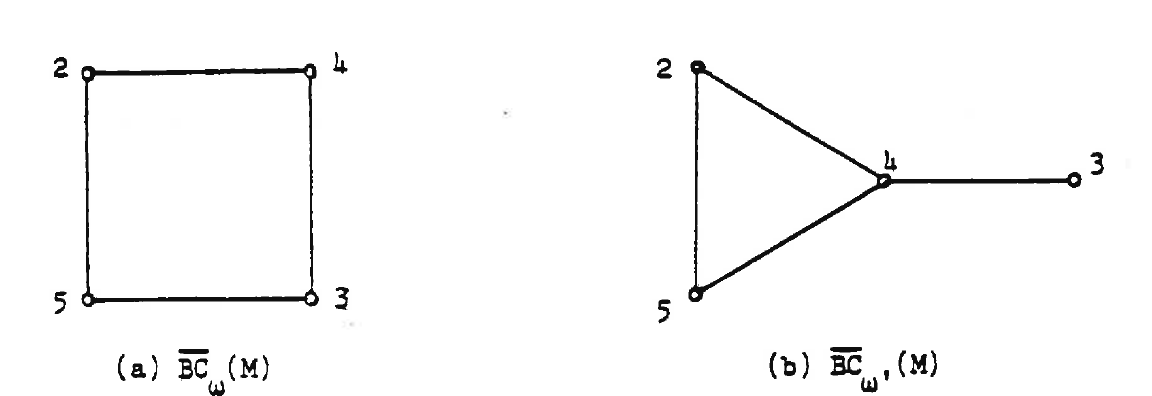
\includegraphics[width=.85\textwidth]{images/fig4.png}\par 图4\end{center}
现在转向壳多项式及计数性质。设 $B$ 是nbc基且 $b\in B$。若 $B-b$ 包含于字典序更小的nbc基，则如(7.9)，$b\in\IP(B)$。反之若 $b$ 内被动，则 $B-b$ 包含于某个先于 $B$ 的基；命题7.4.2的证明说明，包含 $B-b$ 的最早基是nbc基。因此在断路复形的字典壳序中，
\[\RR(B)=\IP(B).\tag{7.14}\]
故壳多项式等于对nbc基求和的 $\sum_Bx^{i(B)}$。而 $B$ 不含断路当且仅当 $e(B)=0$，所以
\[h_{\BC_\omega(M)}(x)=T_M(x,0).\tag{7.15}\]
类似推理可直接得到，或由命题7.4.2(iii)、习题7.2.1及(7.15)得到，约化断路复形的壳多项式为
\[h_{\overline{\BC}_\omega(M)}(x)=\frac1xT_M(x,0).\tag{7.16}\]
\src{13}
由(7.15)，断路复形的面数与次序无关。例7.4.4中两个不同构复形的 $f$ 向量都是 $(1,5,8,4)$。
断路复形的面数及面枚举多项式 $T_M(1+\lambda,0)$ 是拟阵理论中十分有趣的数值不变量。以下假定读者熟悉秩 $r$ 几何格的Möbius函数 $\mu(x,y)$ 和特征多项式
\[p(L;\lambda)=\sum_{x\in L}\mu(\hat0,x)\lambda^{r-r(x)}=\sum_{k=0}^rw_k\lambda^{r-k}.\]
参见 White (1987) 第7、8章或 Stanley (1986)。非负整数 $\widetilde w_k=(-1)^kw_k$ 称为（无符号的）\textbf{第一类Whitney数}。
\st{命题7.4.5}设 $M(S,\omega)$ 是无环有序拟阵，$L$ 是相应几何格。对 $x\in L$，令 $\nbc(x)=\{A\in\BC_\omega(M):\bar A=x\}$，则
\[|\nbc(x)|=(-1)^{r(x)}\mu(\hat0,x).\]
\pr 证明 $(-1)^{r(y)}|\nbc(y)|$ 与 $\mu(\hat0,y)$ 满足同一递推。仅空集张成空平坦集，故 $|\nbc(\hat0)|=1$。设 $x\ne\hat0$，令 $S'$ 为平坦集 $x$ 上的点集，$M'(S',\omega')$ 为相应限制。$S'$ 的子集在 $M'$ 中为断路当且仅当在 $M$ 中为断路。因此 $\BC_{\omega'}(M')=\bigcup_{y\le x}\nbc(y)$，且为无交并。$\nbc(y)$ 的每个元素既独立又张成 $y$，故基数为 $r(y)$。又因 $\BC_{\omega'}(M')$ 是锥，由(7.2)，
\[\sum_{\hat0\le y\le x}(-1)^{r(y)}|\nbc(y)|=-\chi(\BC_{\omega'}(M'))=0.\]
证明完成。\qed
把命题两侧对秩为 $k$ 的平坦集求和，左边得到无断路 $k$ 元子集总数，右边得到 $\widetilde w_k$。于是：
\st{定理7.4.6}无环拟阵的第一类Whitney数，等于任意次序诱导的断路复形的面数。
结合(7.15)和命题7.2.3，可写为
\[p(M;\lambda)=(-1)^rh_{\BC_\omega(M)}(1-\lambda)=(-1)^rT_M(1-\lambda,0).\tag{7.17}\]
例7.3.5中，已算得 $T_M(x,y)=x^3+2x^2+y^2+2xy+x+y$，所以 $T_M(1-\lambda,0)=4-8\lambda+5\lambda^2-\lambda^3=-p(M;\lambda)$。这与其断路复形的 $f$ 向量 $(1,5,8,4)$ 相符。
本节最后确定拟阵复形及（约化）断路复形的欧拉示性数。需要拟阵 $M(S)$ 的\textbf{beta不变量}
\[\beta(M)=(-1)^{r(S)}\sum_{A\subseteq S}(-1)^{|A|}r(A),\tag{7.18}\]
其讨论见 White (1987) 第7章。再定义\textbf{Möbius不变量}
\[\widetilde\mu(M)=\begin{cases}|\mu_L(\hat0,\hat1)|,&M\text{ 无环},\\0,&M\text{ 有环},\end{cases}\tag{7.19}\]
其中第一种情形的 $L$ 是 $M$ 的平坦集格。显然 $\widetilde\mu(M)=\widetilde w_r(L)$。
\src{14}
\st{命题7.4.7}设 $M$ 秩为 $r$，在(ii)、(iii)中还假定无环且按 $\omega$ 排序。则
\begin{enumerate}[label=(\roman*)]
\item $\chi(\IN(M))=(-1)^{r-1}\widetilde\mu(M^*)$；
\item $\chi(\BC_\omega(M))=0$；
\item $\chi(\overline{\BC}_\omega(M))=(-1)^r\beta(M)$。
\end{enumerate}
\pr (ii)由锥性质立即得到。其余用推论7.2.4的 $\chi(\Delta)=(-1)^{r-1}h_\Delta(0)$。对(i)，当 $M^*$ 无环时，(7.12)、(7.17)给出
\[h_{\IN(M)}(0)=T_M(0,1)=T_{M^*}(1,0)=(-1)^{n-r}p(M^*;0)=\widetilde\mu(M^*).\]
若 $M^*$ 有环，则 $\IN(M)$ 是锥，两边都是零。对(iii)，由(7.16)和定理7.3.7，
\[\begin{aligned}
h_{\overline{\BC}_\omega(M)}(0)&=\frac{\partial T_M}{\partial x}(0,0)\\
&=\sum_{A\subseteq S}(r(S)-r(A))(-1)^{r(S)-r(A)-1+r^*(S)-r^*(S-A)}\\
&=(-1)^{r(S)}\sum_{A\subseteq S}(r(A)-r(S))(-1)^{|A|}=\beta(M).
\end{aligned}\]\qed
由此对所有拟阵有 $\beta(M)\ge0$。为后续使用，列出下述性质；证明见 White (1987) 第7章。
\st{命题7.4.8}对任意 $|S|\ge2$ 的拟阵 $M(S)$：(i) $\beta(M)=\beta(M^*)$；(ii) $\beta(M)>0$ 当且仅当 $M$ 连通。
